\subsection{General information}
\begin{frame}
	\frametitle{Proton Accelerator at Paul Scherrer Institute (PSI)}
	\begin{itemize}
		\setlength{\itemsep}{\fill}
		\item High Intensity Proton Accelerator (HIPA) at PSI (Cyclotron)
		\item \SI{590}{\mega\electronvolt} proton beam with beam current up to \SI{2.4}{\milli\ampere}
		\begin{itemize}
			\vspace*{4pt}
			\item \SI{\sim1.4}{\mega\watt} \ra most powerful proton accelerator in the world
		\end{itemize}
		\vspace*{4pt}
		\item only two comparable accelerators
		\begin{itemize}
			\vspace*{4pt}
			\item TRIUMF in Vancouver (\SI{\sim0.25}{\mega\watt})
			\item LAMPF in Los Alamos (\SI{\sim0.8}{\mega\watt})
		\end{itemize}
		\item LHC takes \SI{28}{\minute} to accelerate a full injection (\SI{\sim0.2}{\mega\watt})
	\end{itemize}
	\begin{figure}
		\centering
		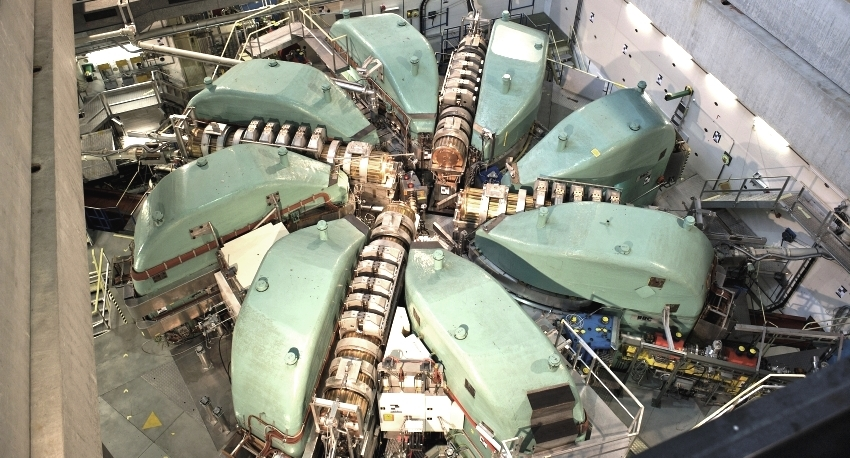
\includegraphics[width=6.5cm]{cyclotron}
	\end{figure}
\end{frame}
% ============================ new frame ==========================================>
\begin{frame}
	\frametitle{Beam line at Paul Scherrer Institute (PSI)}
	\begin{minipage}[c][.6\textheight]{6.5cm}
		\begin{itemize}
			\setlength{\itemsep}{\fill}
			\item using beam line $\uppi$M1 with \SI{260}{\mega\electronvolt\per c} positive pions ($\uppi^+$)
			\item tunable particle fluxes from \SI{2}{\kilo\hertz\per cm^2} to \SI{10}{\mega\hertz\per cm^2}
		\end{itemize}
		\begin{figure}
			\centering
			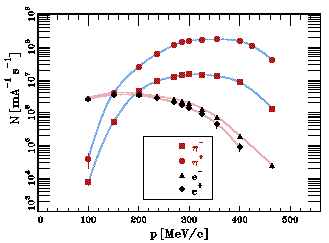
\includegraphics[width=5cm]{pim1}
		\end{figure}
	\end{minipage}
	\begin{minipage}{4.5cm}
		\begin{figure}
			\centering
			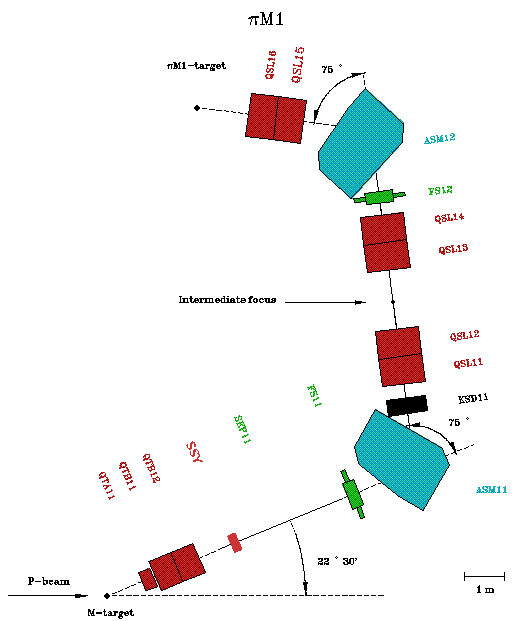
\includegraphics[width=5cm]{bpim1}
		\end{figure}
	\end{minipage}
\end{frame}
% ============================ new frame ==========================================>
\begin{frame}
	\frametitle{Measurements}
	\begin{itemize}
		\item performing several beam tests starting in $2013$
		\item using a modular self-built beam telescope with two possible setups:
			\begin{itemize}
				\item pad setup (testing whole diamonds as single pad detector)
				\item pixel setup (testing diamond sensors implanted on CMS-Pixel Chips)
			\end{itemize}
		\item investigating several materials and devices
		\begin{itemize}
			\item scCVD pad detectors (reproduce rate effect)
			\item pCVD pad and pixel detectors
			\item very first 3D pixel detector
		\end{itemize}
		\item studying non-irradiated and irradiated devices (up to \SI{1e16}{neq\per cm^2})
	\end{itemize}
	\begin{figure}
		\centering
		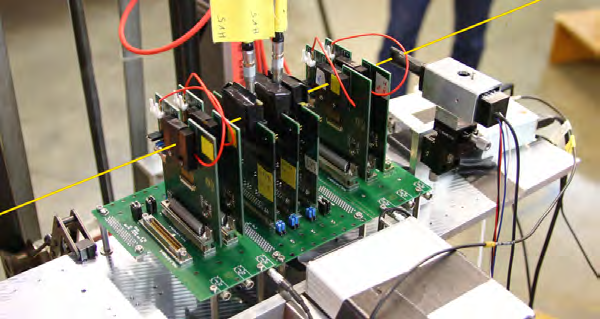
\includegraphics[width=6cm]{pad}
	\end{figure}
\end{frame}
% ============================ new frame ==========================================>
\subsection{Setup}
\begin{frame}
	\frametitle{Setup}
	\begin{figure}
		\centering
		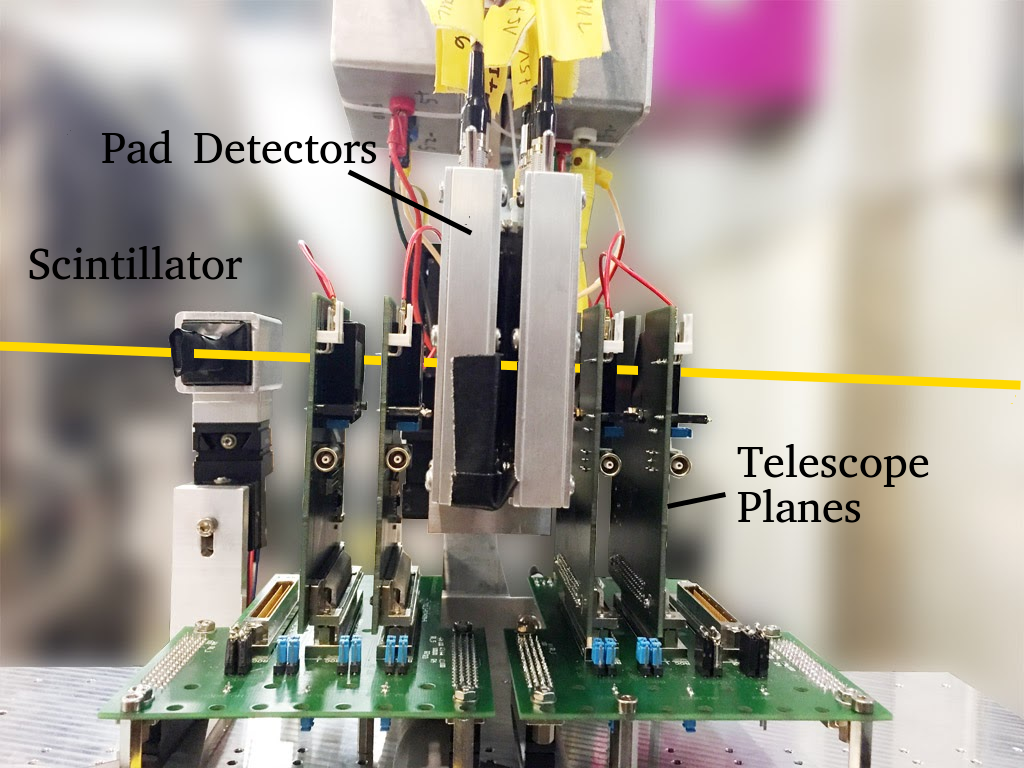
\includegraphics[width=5.5cm]{Setup}
	\end{figure}
	\begin{itemize}
		\setlength{\itemsep}{\fill}
		\item 4 tracking planes with analogue CMS pixel chips
		\item 2 diamond pad detectors
		\item scintillator for precise trigger timing: sigma of \SI{1.3\pm.1}{ns}
		\item resolution: \SI{\sim80x50}{\micro\meter}
	\end{itemize}
\end{frame}
% ============================ new frame ==========================================>
\begin{frame}
	\frametitle{Schematics}
	\begin{figure}
		\centering
		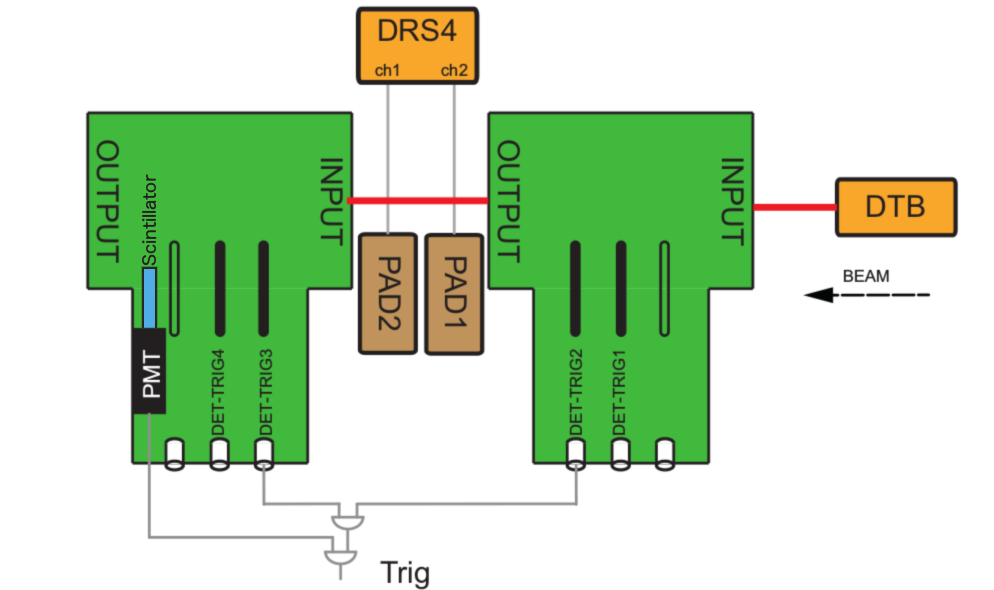
\includegraphics[width=7cm]{SchematicsV2}
	\end{figure}
	\begin{itemize}
		\setlength{\itemsep}{\fill}
		\item using PSI DRS4 Evaluation Board as digitizer for the pad waveforms
		\item using Digital Test Board (DTB) and pXar software for the telescope readout
		\item global trigger as coincidence of fastOR self trigger and scintillator signal
		\item EUDAQ as DAQ framework
	\end{itemize}
\end{frame}
% ============================ new frame ==========================================>
\begin{frame}
	\frametitle{DAQ}
	\begin{figure}
		\centering
		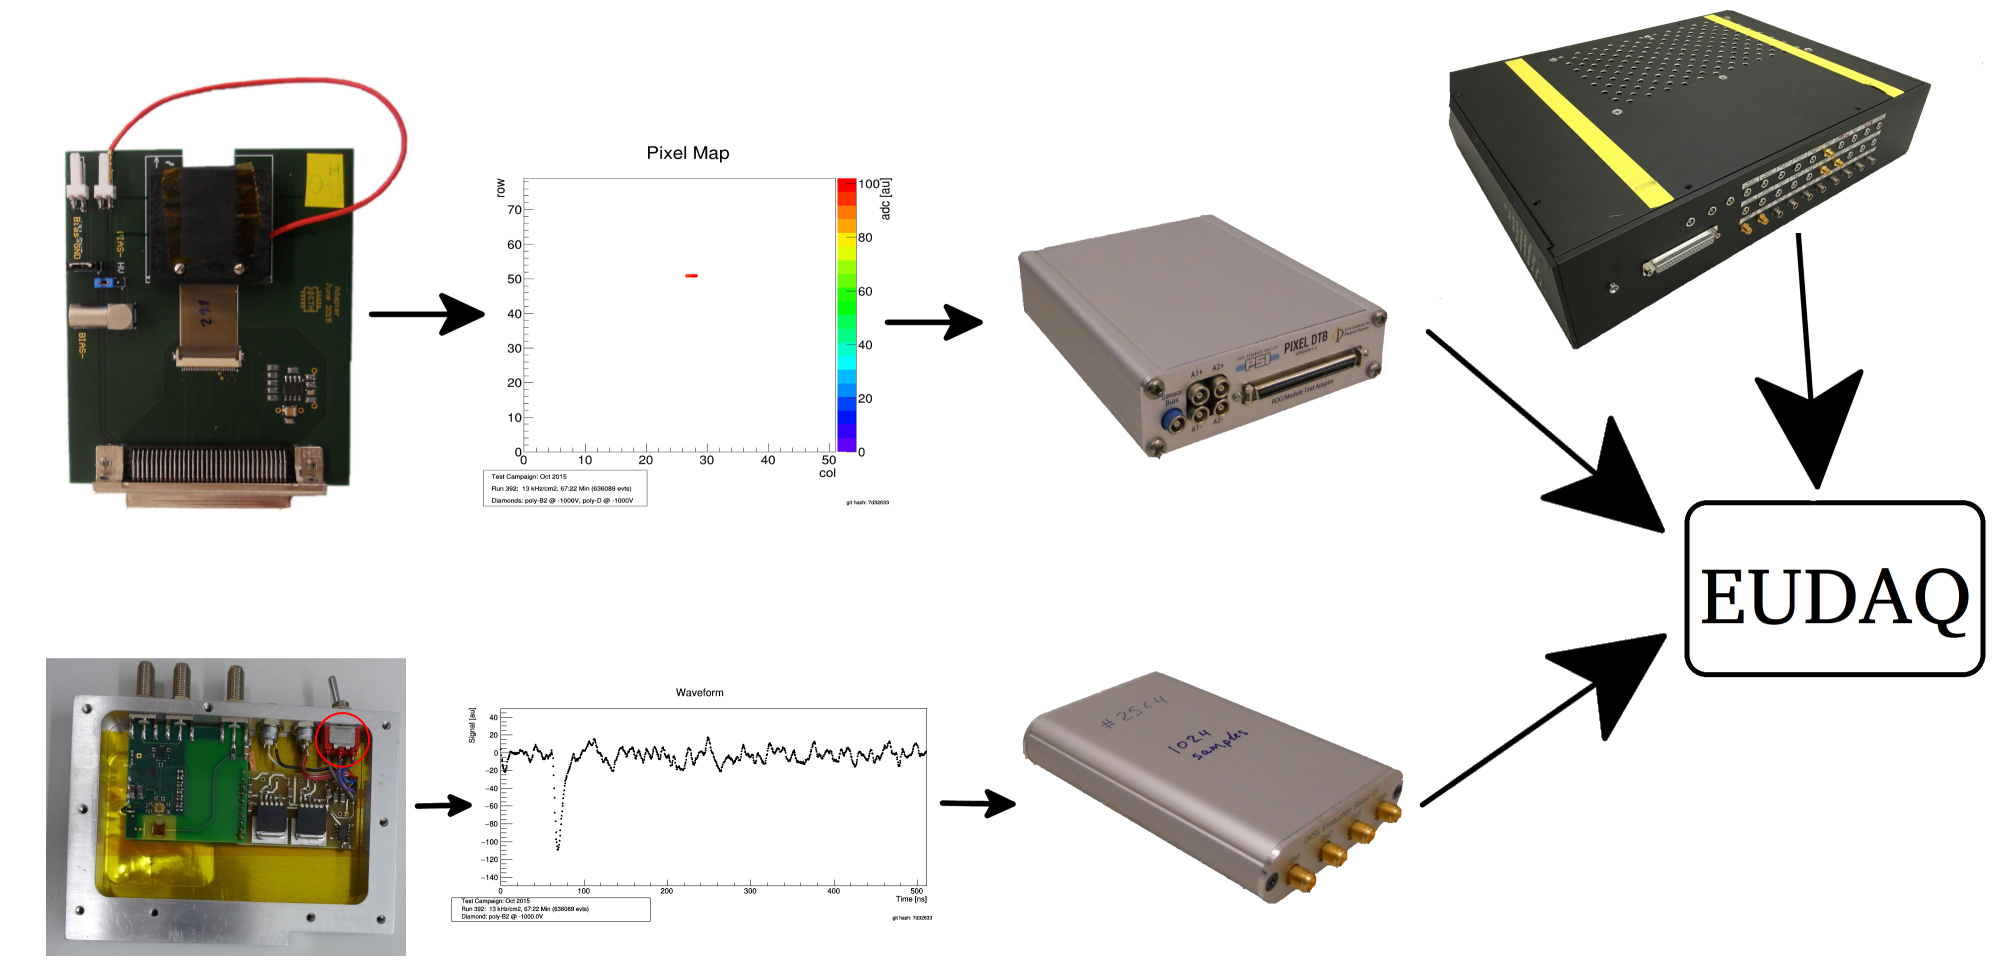
\includegraphics[width=.8\textwidth]{Intro}
	\end{figure}
	\begin{itemize}
		\item custom-built trigger unit to process the single triggers and provide global one for all devices
		\item saving event based data stream as binary file using EUDAQ
	\end{itemize}
\end{frame}
% ============================ new frame ==========================================>
\subsection{Analysis and Results}
\begin{frame}
	\frametitle{Waveforms}
	\vspace*{-20pt}
	\begin{center}
		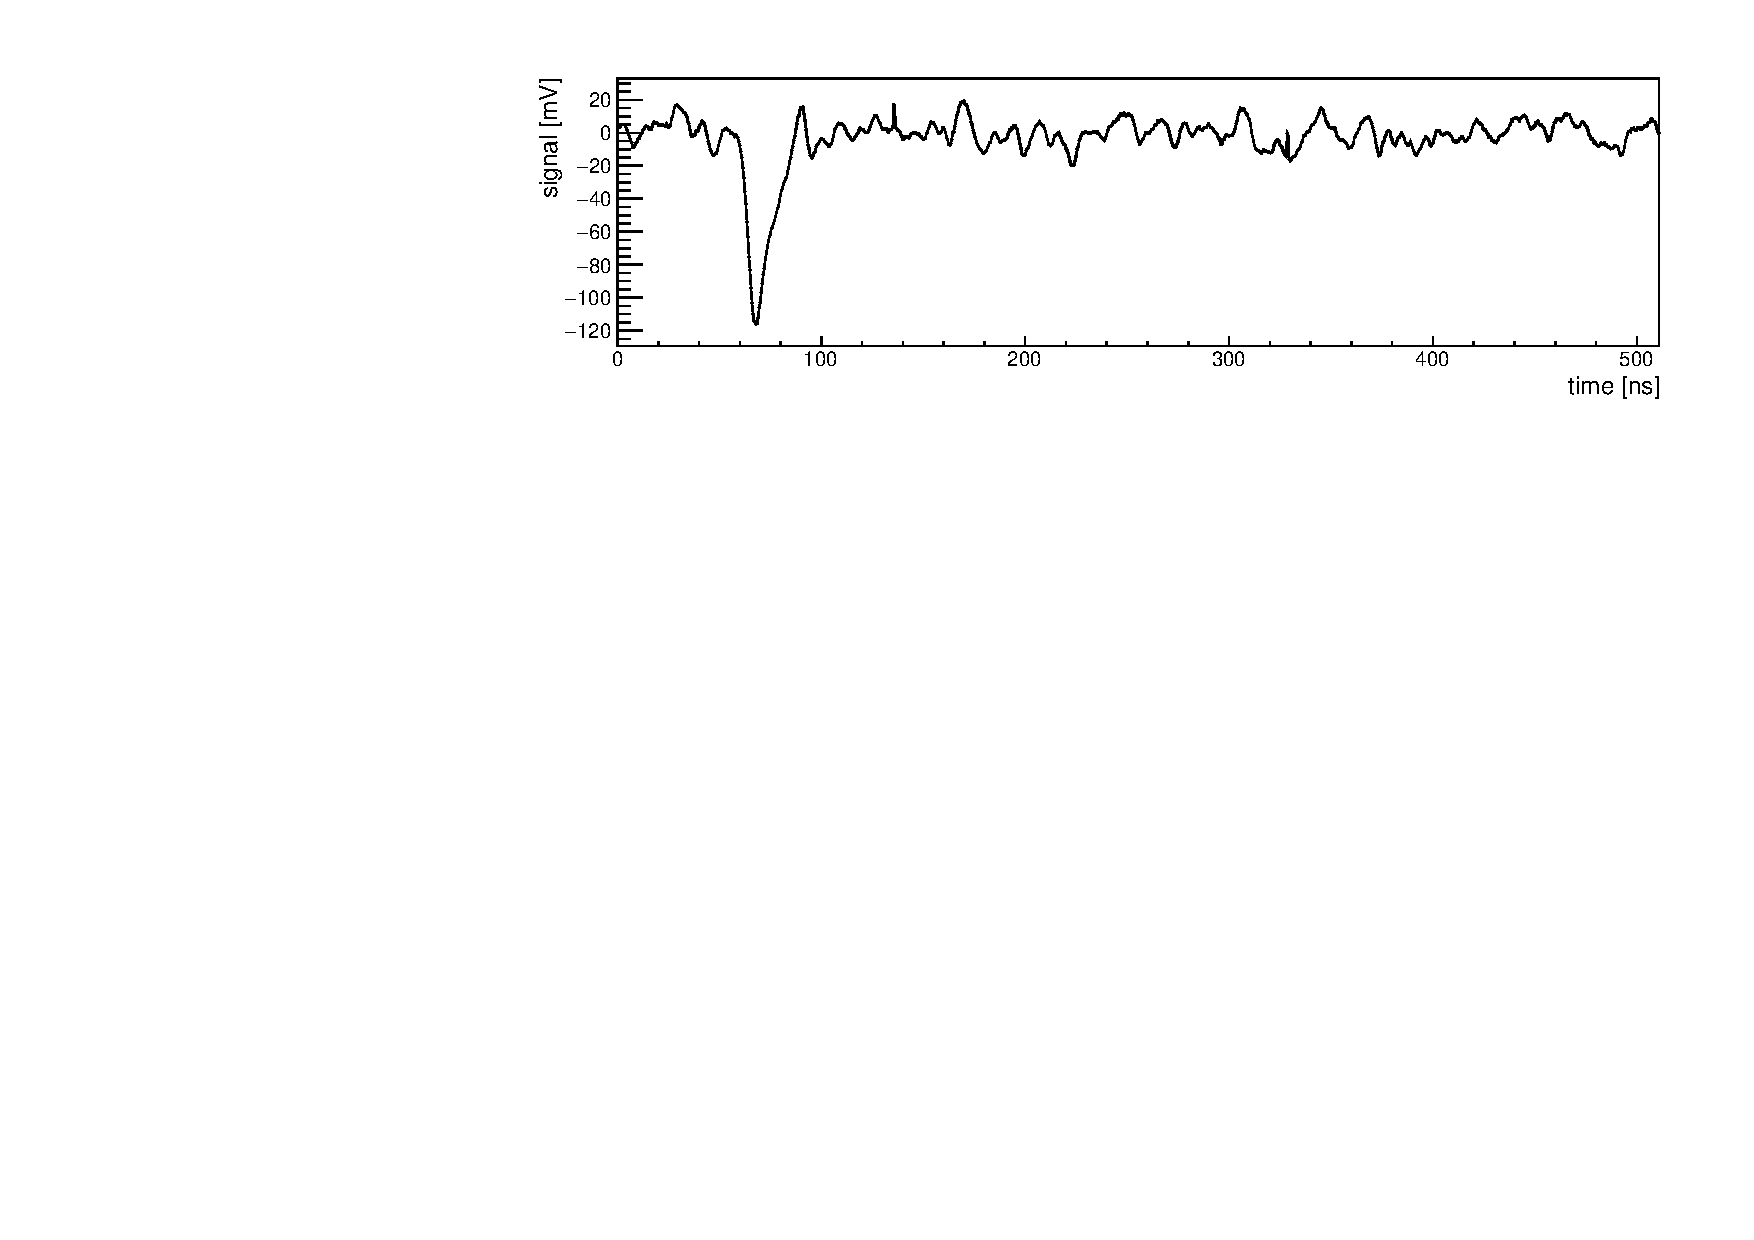
\includegraphics[angle=270, width=.7\textwidth]{SignalWaveform}\\
		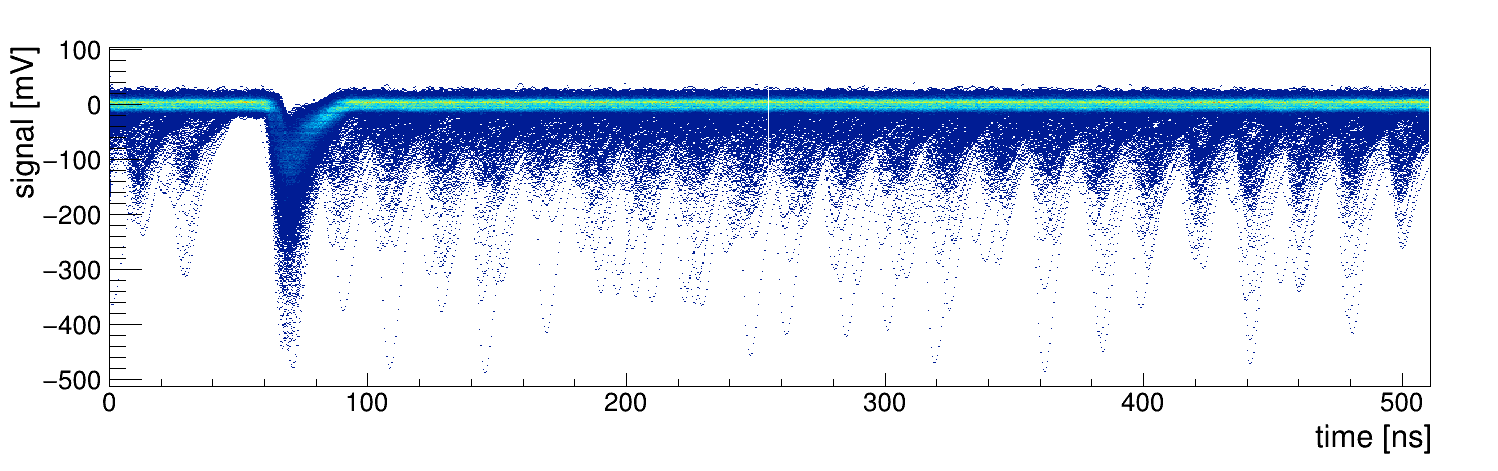
\includegraphics[width=.7\textwidth]{SignalWaveforms5000}
	\end{center}
	\begin{itemize}
		\item most frequented peak (\SI{\sim70}{ns}): triggered signal
		\item other peaks originate from other buckets ($\rightarrow$ resolve beam structure of \SI{\approx19.7}{ns})
		\item system does not allow signals in pre-signal bucket due to fastOR trigger deadtime
	\end{itemize}
\end{frame}
% ============================ new frame ==========================================>
\begin{frame}
	\frametitle{Pulse Height Calculation}
	\begin{center}
		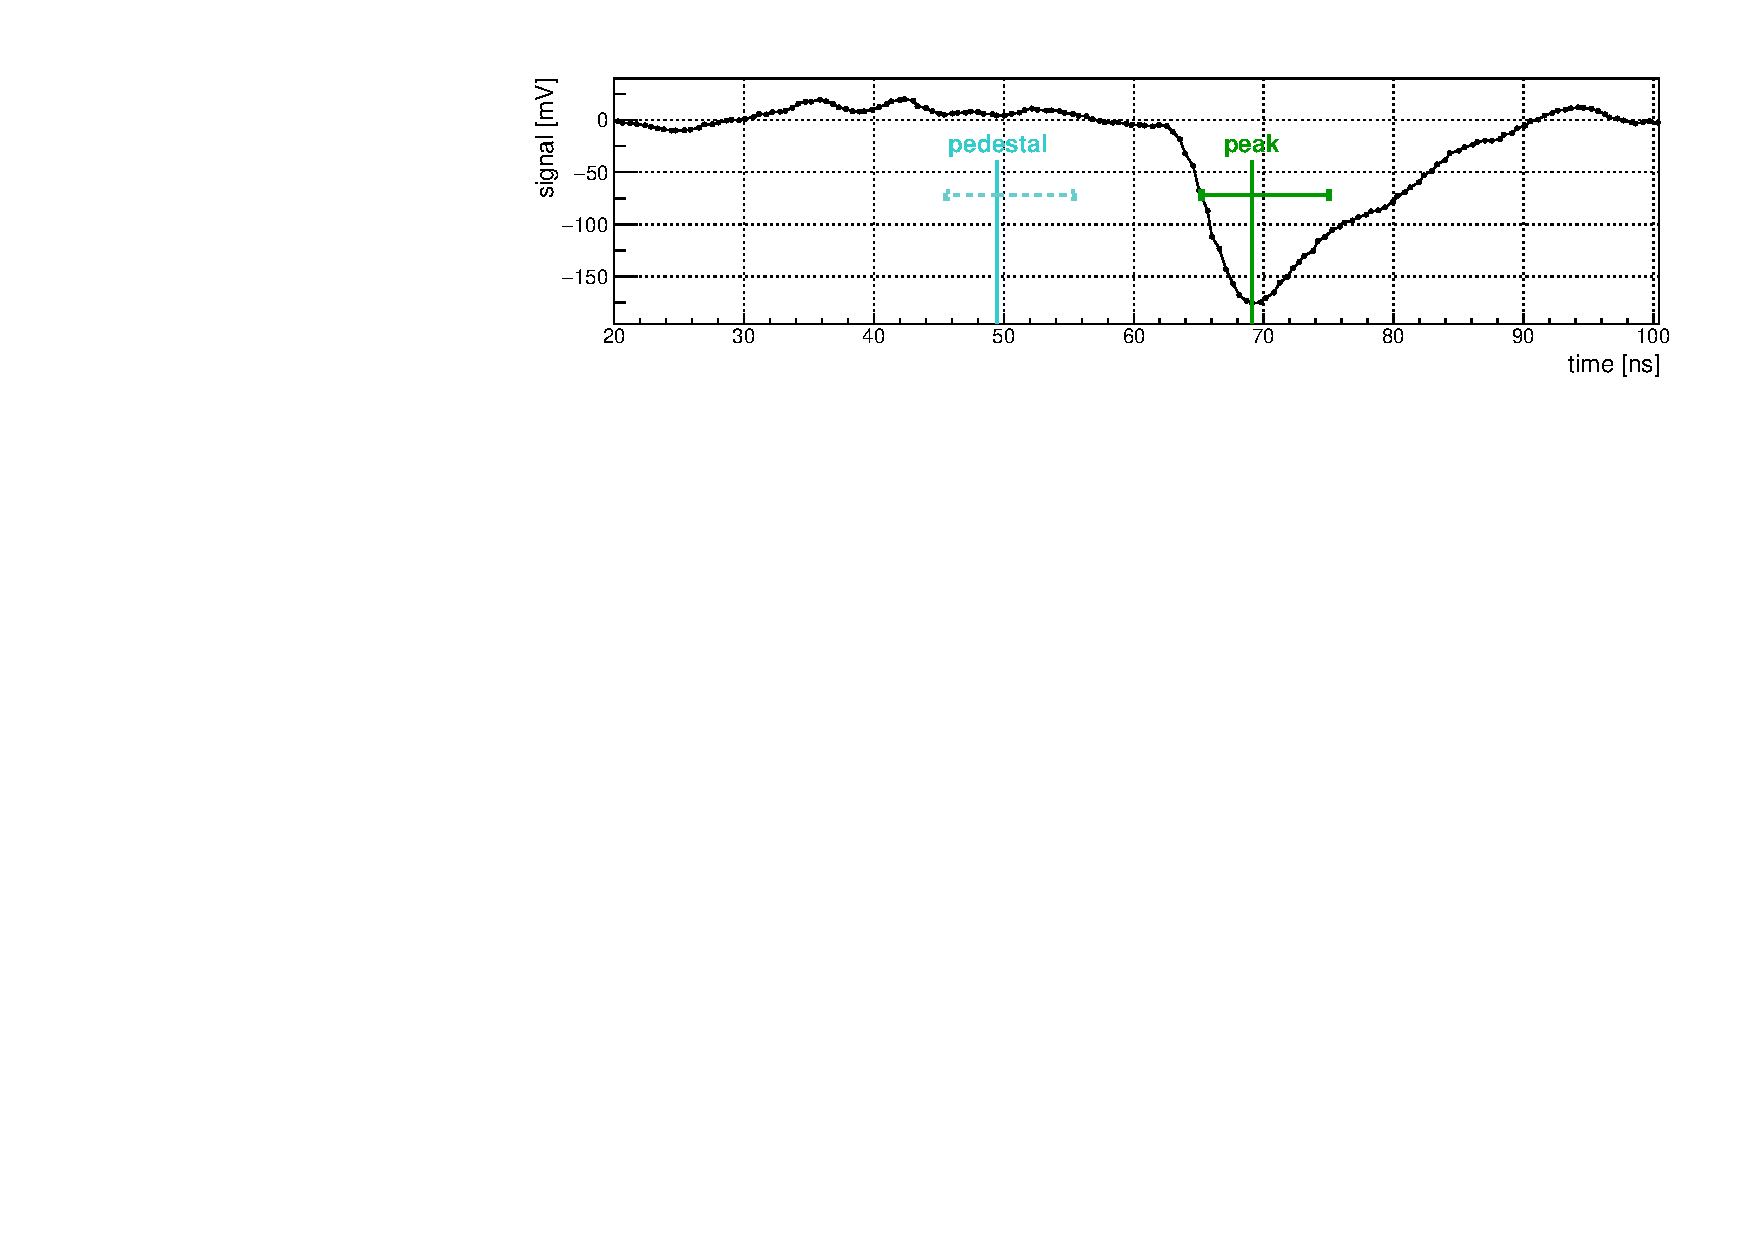
\includegraphics[angle=270, width=.8\textwidth]{intpeaks}\\
	\end{center}
	\begin{itemize}
		\setlength{\itemsep}{\fill}
		\item finding the peak in the signal region
		\item integrating the signal in time fixed asymmetric integral around peak
		\item same integration for pedestal (base line $\rightarrow$ noise)
		\item optimising the integral width by highest SNR (Integral / Pedestal Sigma)
		\item subtracting the pedestal from the signal integral on event-wise basis 
	\end{itemize}
\end{frame}
% ============================ FRAME 18 ==========================================>
\begin{frame}
	\frametitle{Pulse Height Distribution and Signal Maps}
	\vspace*{-7.5pt}
	\def \sp {0.65\textwidth}
	\begin{figure}
		\centering
		\begin{subfigure}{0.45\textwidth} 
			\centering 
			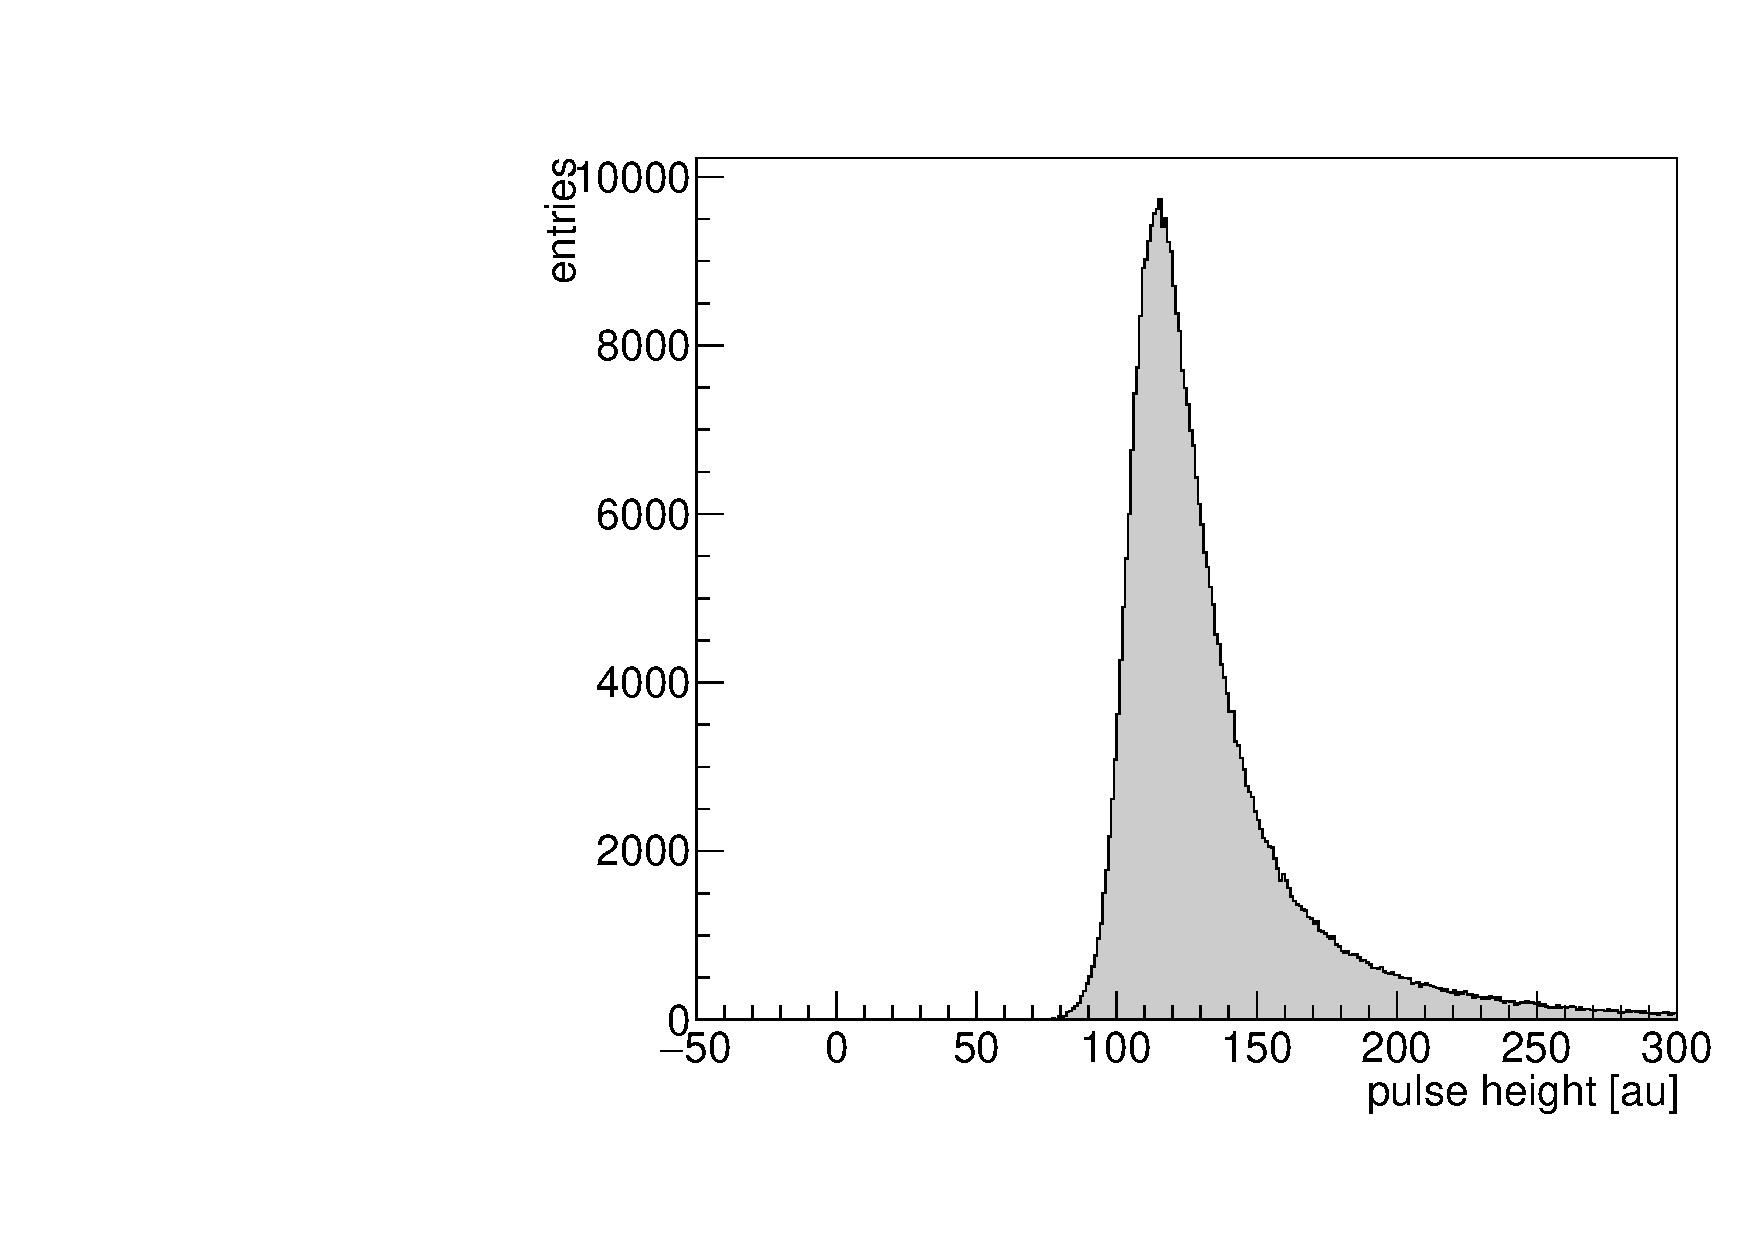
\includegraphics[angle=270, width=\sp]{sDisto}
		\end{subfigure}
		\begin{subfigure}{0.45\textwidth} 
			\centering 
			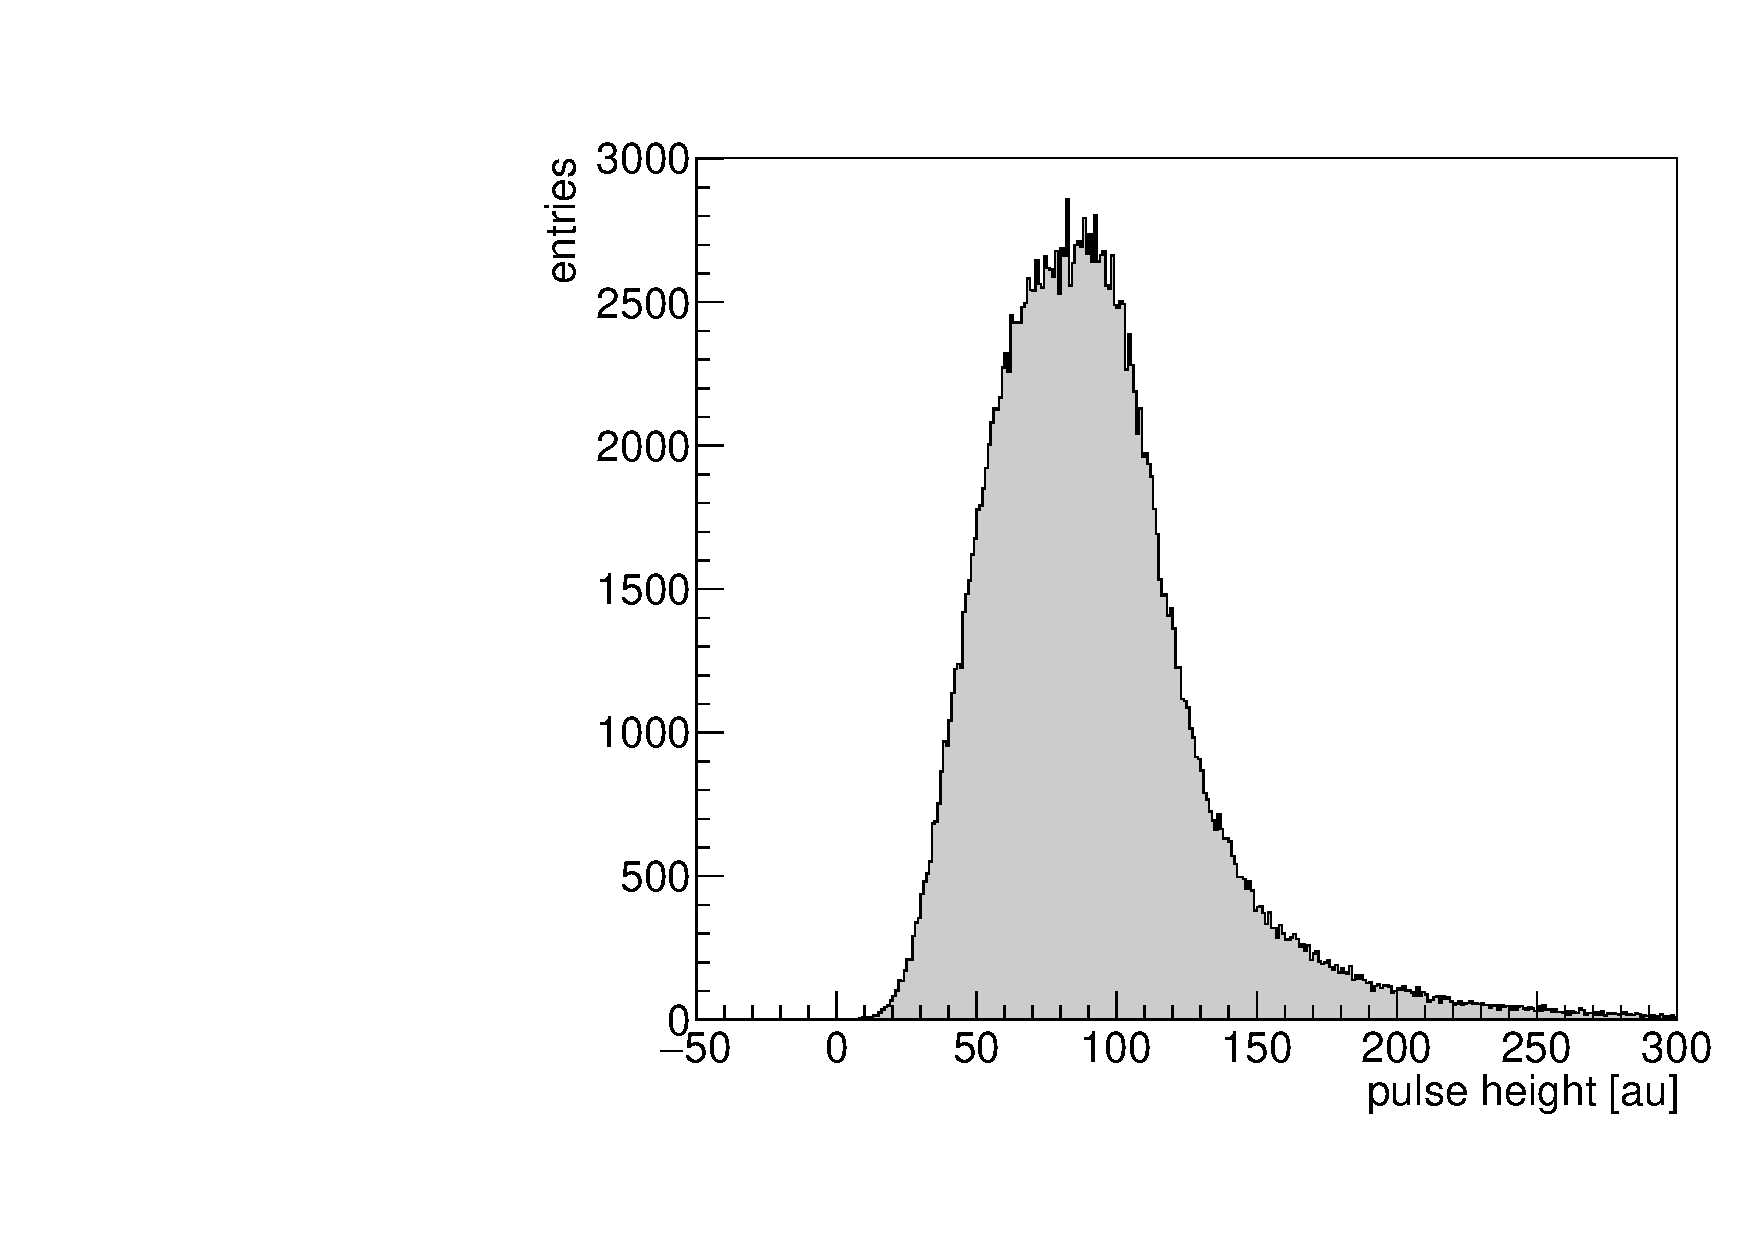
\includegraphics[angle=270, width=\sp]{pDisto}
		\end{subfigure}
	\end{figure}
	\vspace*{-15pt}
	\begin{figure}
	\centering
		\begin{subfigure}{0.45\textwidth} 
			\centering 
			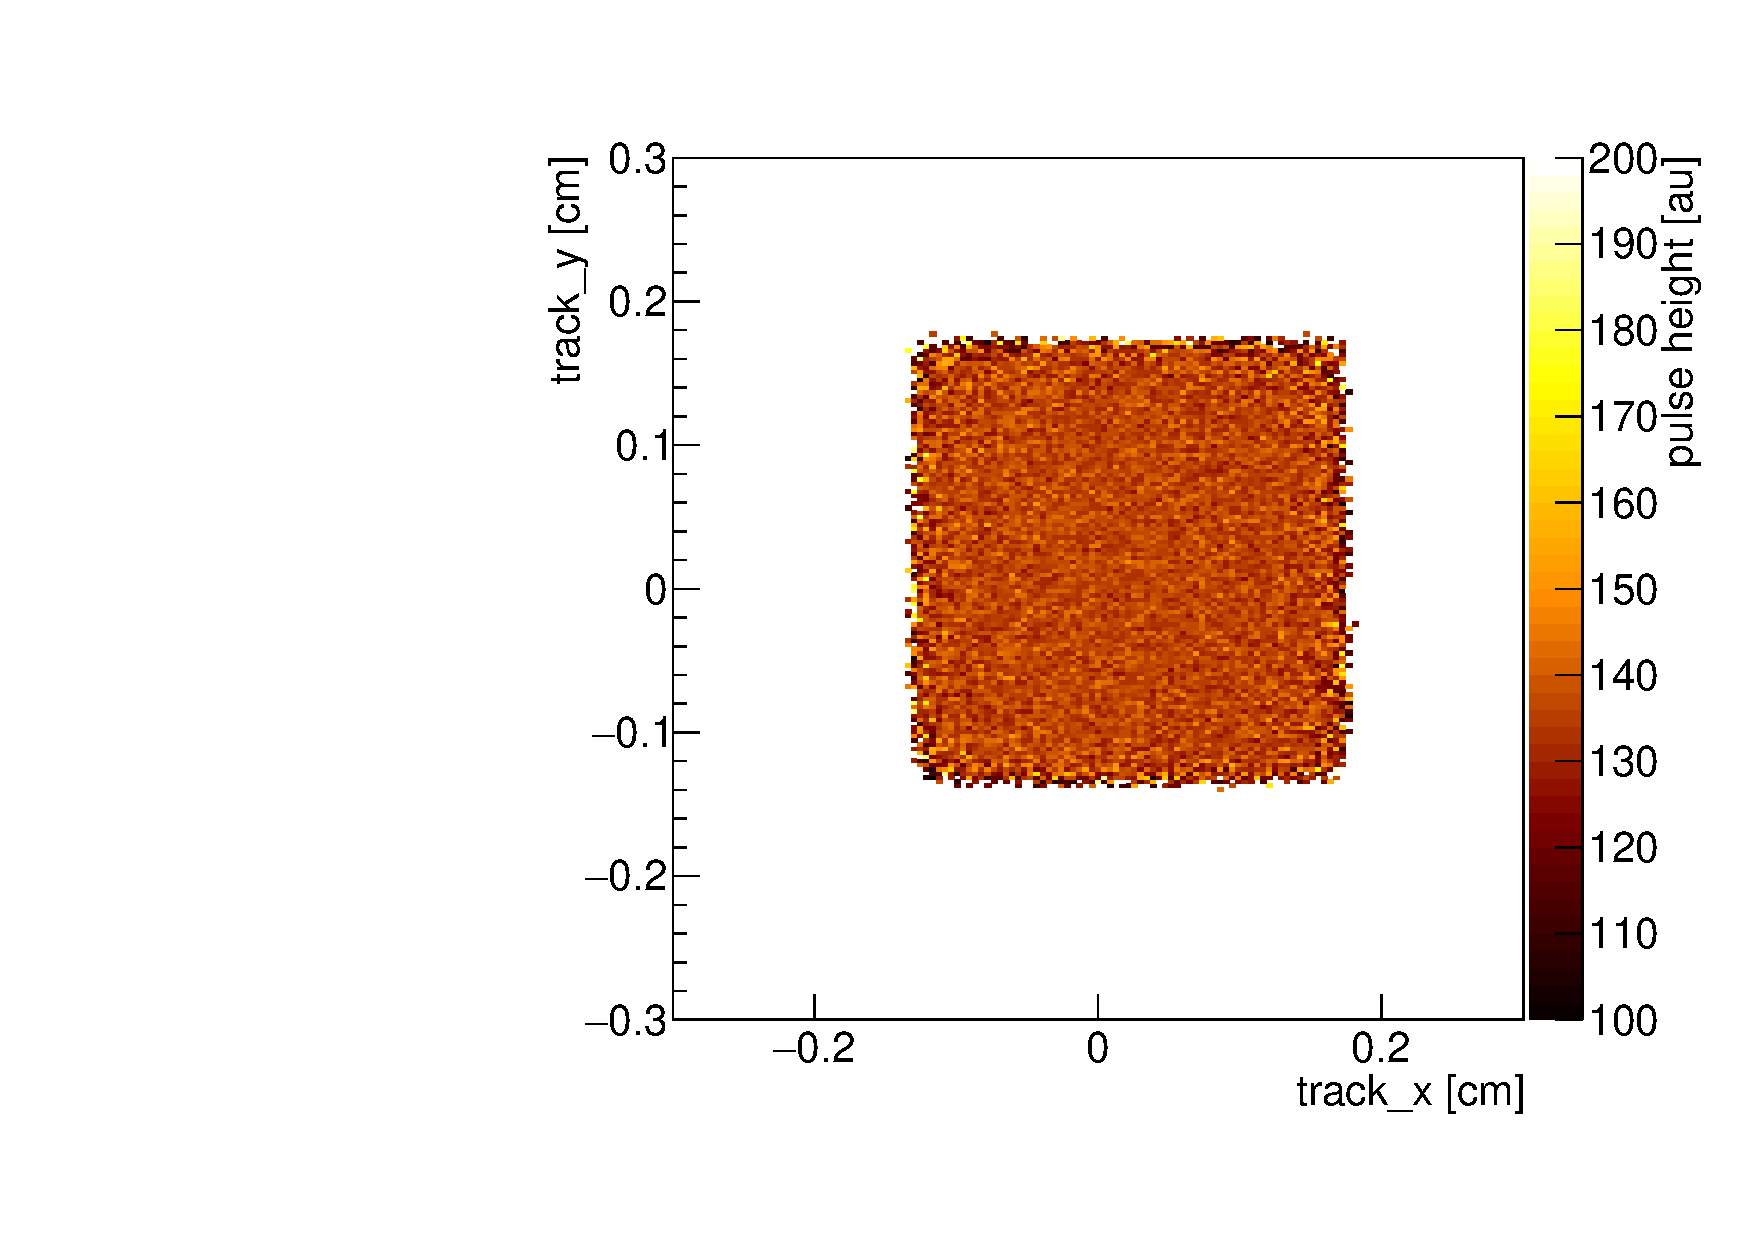
\includegraphics[angle=270, width=\sp]{sSigMap}
			\caption{single-crystalline}
		\end{subfigure}
		\begin{subfigure}{0.45\textwidth} 
			\centering 
			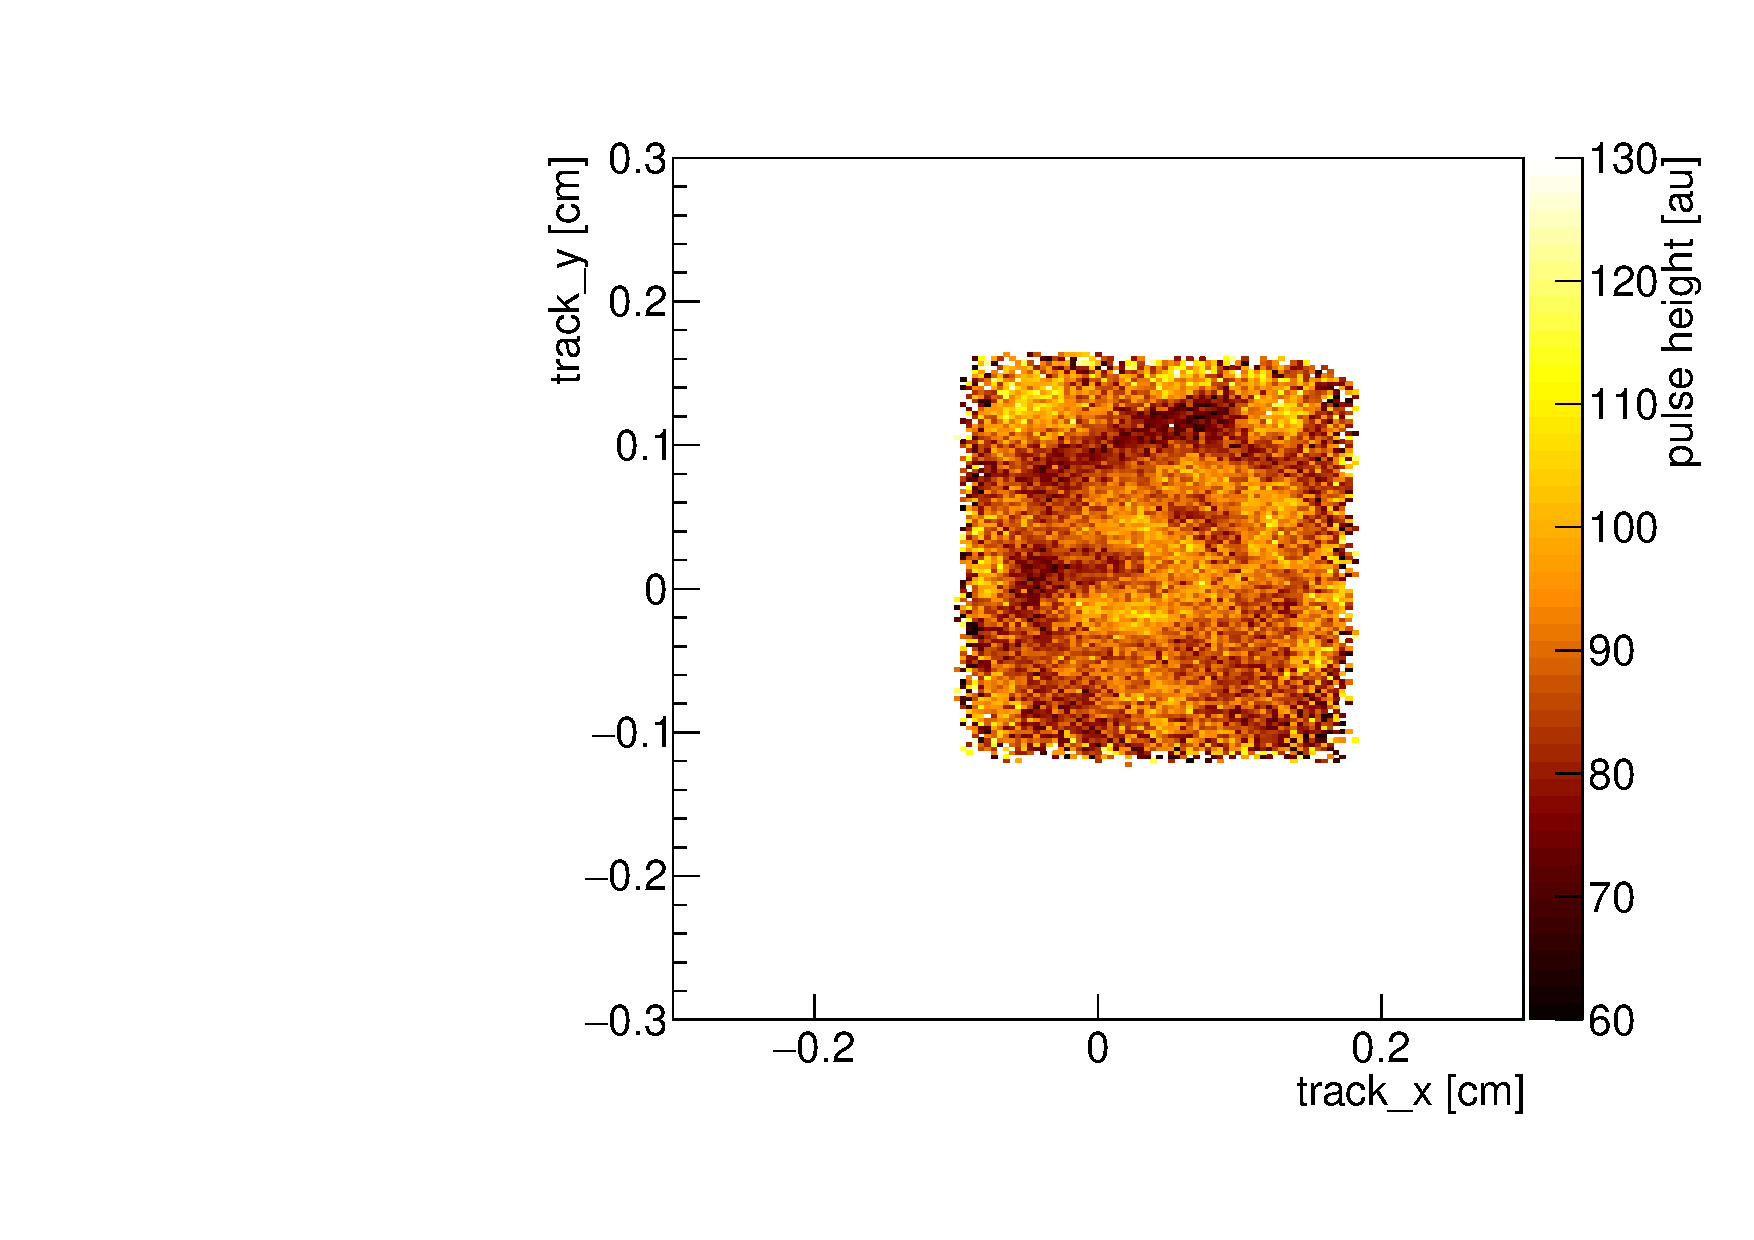
\includegraphics[angle=270, width=\sp]{pSigMap}
			\caption{poly-crystalline}
		\end{subfigure} 
	\end{figure}
\end{frame}
% ============================ new frame ==========================================>
\begin{frame}
	\frametitle{Signal vs. Particle Flux}
	\begin{minipage}[c][.75\textheight]{.5\textwidth}
		\begin{itemize}
			\setlength{\itemsep}{\fill}
			\item after all analysis steps: look for rate dependence of pCVD diamonds
			\item found diamond pad detectors that show no or very little dependence on rate
			\item no dependence up to \SI{1e16}{neq\per cm^2}
			\item large systematic errors due to reproducibility
		\end{itemize}
		\vspace*{3pt}
		\textbf{To do:}
		\begin{itemize}
			\setlength{\itemsep}{\fill}
			\item test higher irradiated samples
			\item improve reproducibility
			\item prove the same for pixel detectors
		\end{itemize}
	\end{minipage}
	\hspace*{5pt}
	\begin{minipage}{.45\textwidth}
		\begin{figure}
			\centering
			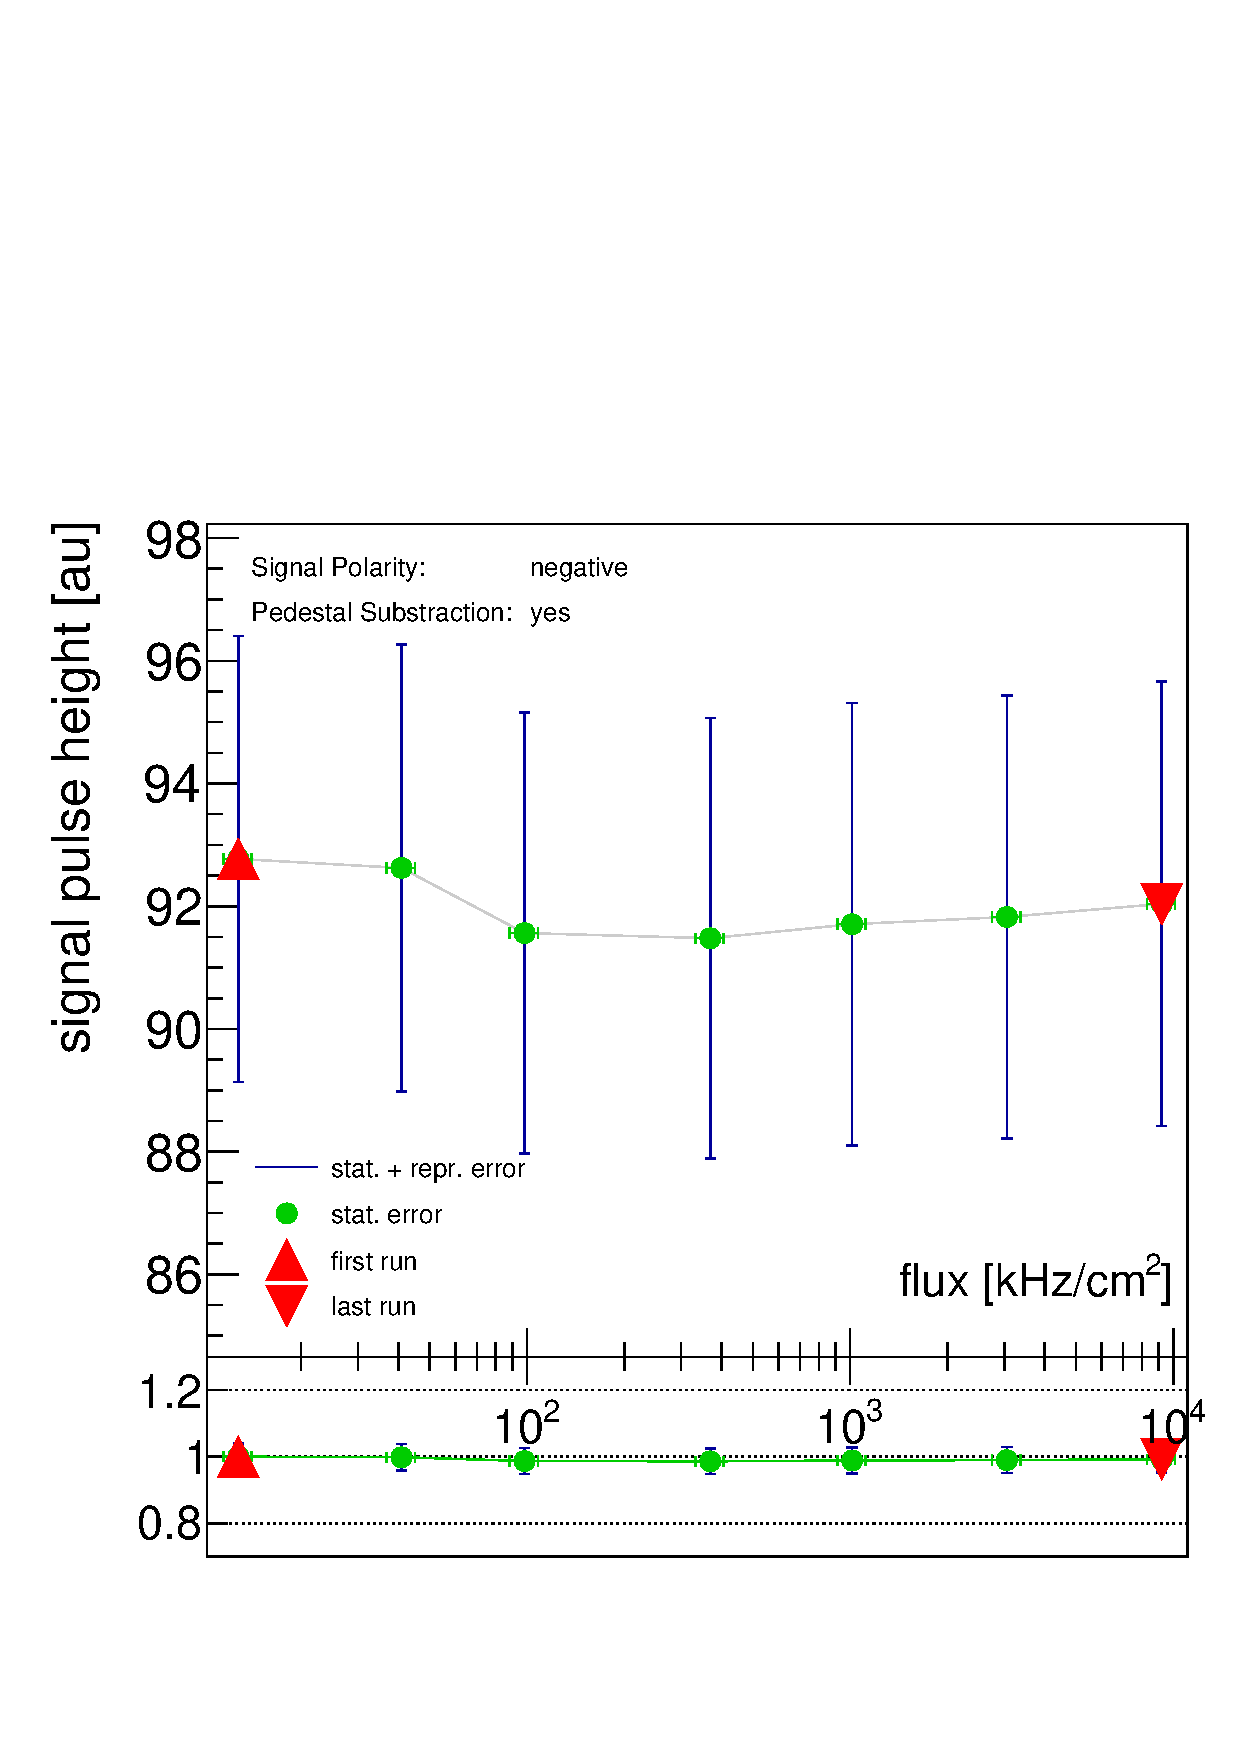
\includegraphics[width=\textwidth]{rateplot}
		\end{figure}
	\end{minipage}
\end{frame}
